\begin{figure}[htbp]
\centering
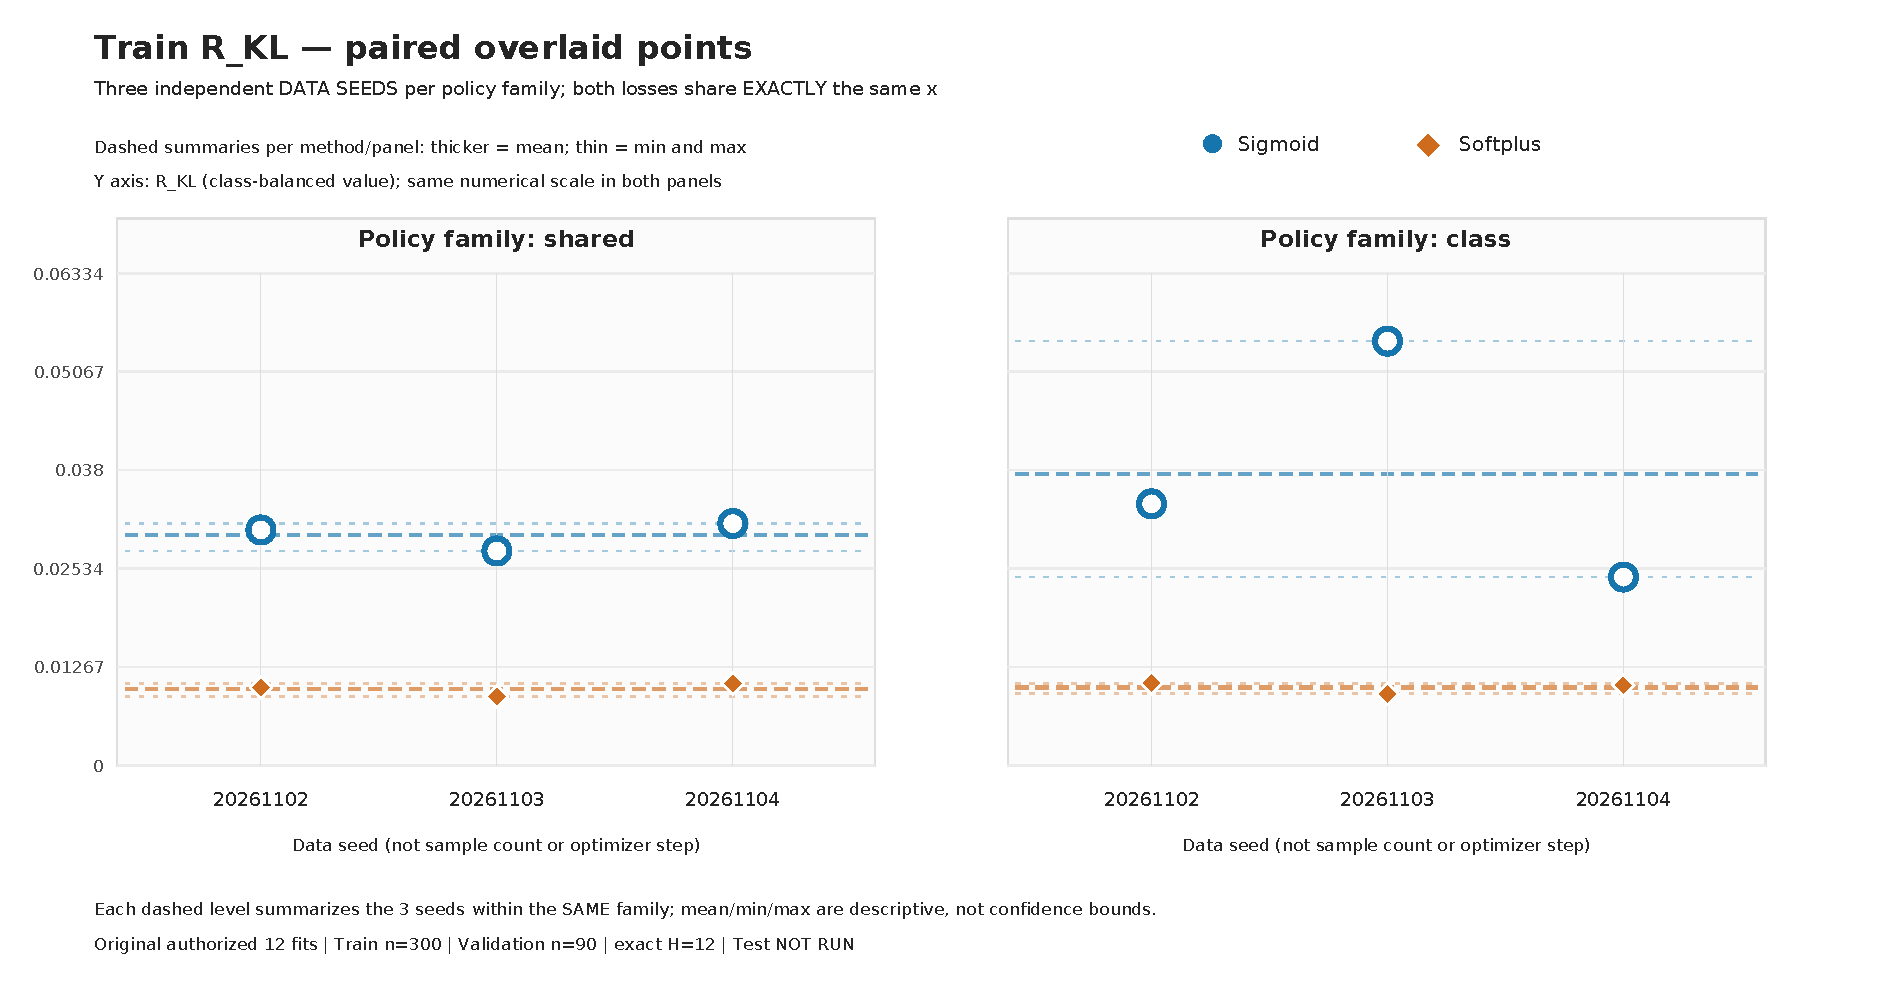
\includegraphics[width=0.98\linewidth]{code/experiments/ch4_loss_controlled_comparison/figures/phase2_tex/phase2_train_R_KL_six_pairs.pdf}
\caption{تراکم مبتنی بر واگرایی کولبک--لایبلر در مجموعه آموزش، با هم‌مکانی افقی دو روش در هر بذر و خطوط چین کمینه، میانگین و بیشینه هر روش و خانواده سیاست. مقادیر کمتر به معنای تراکم بیشتر حول مراکز کلاس است.}
\label{fig:ch4-e13-train-r_kl}
\end{figure}

\begin{figure}[htbp]
\centering
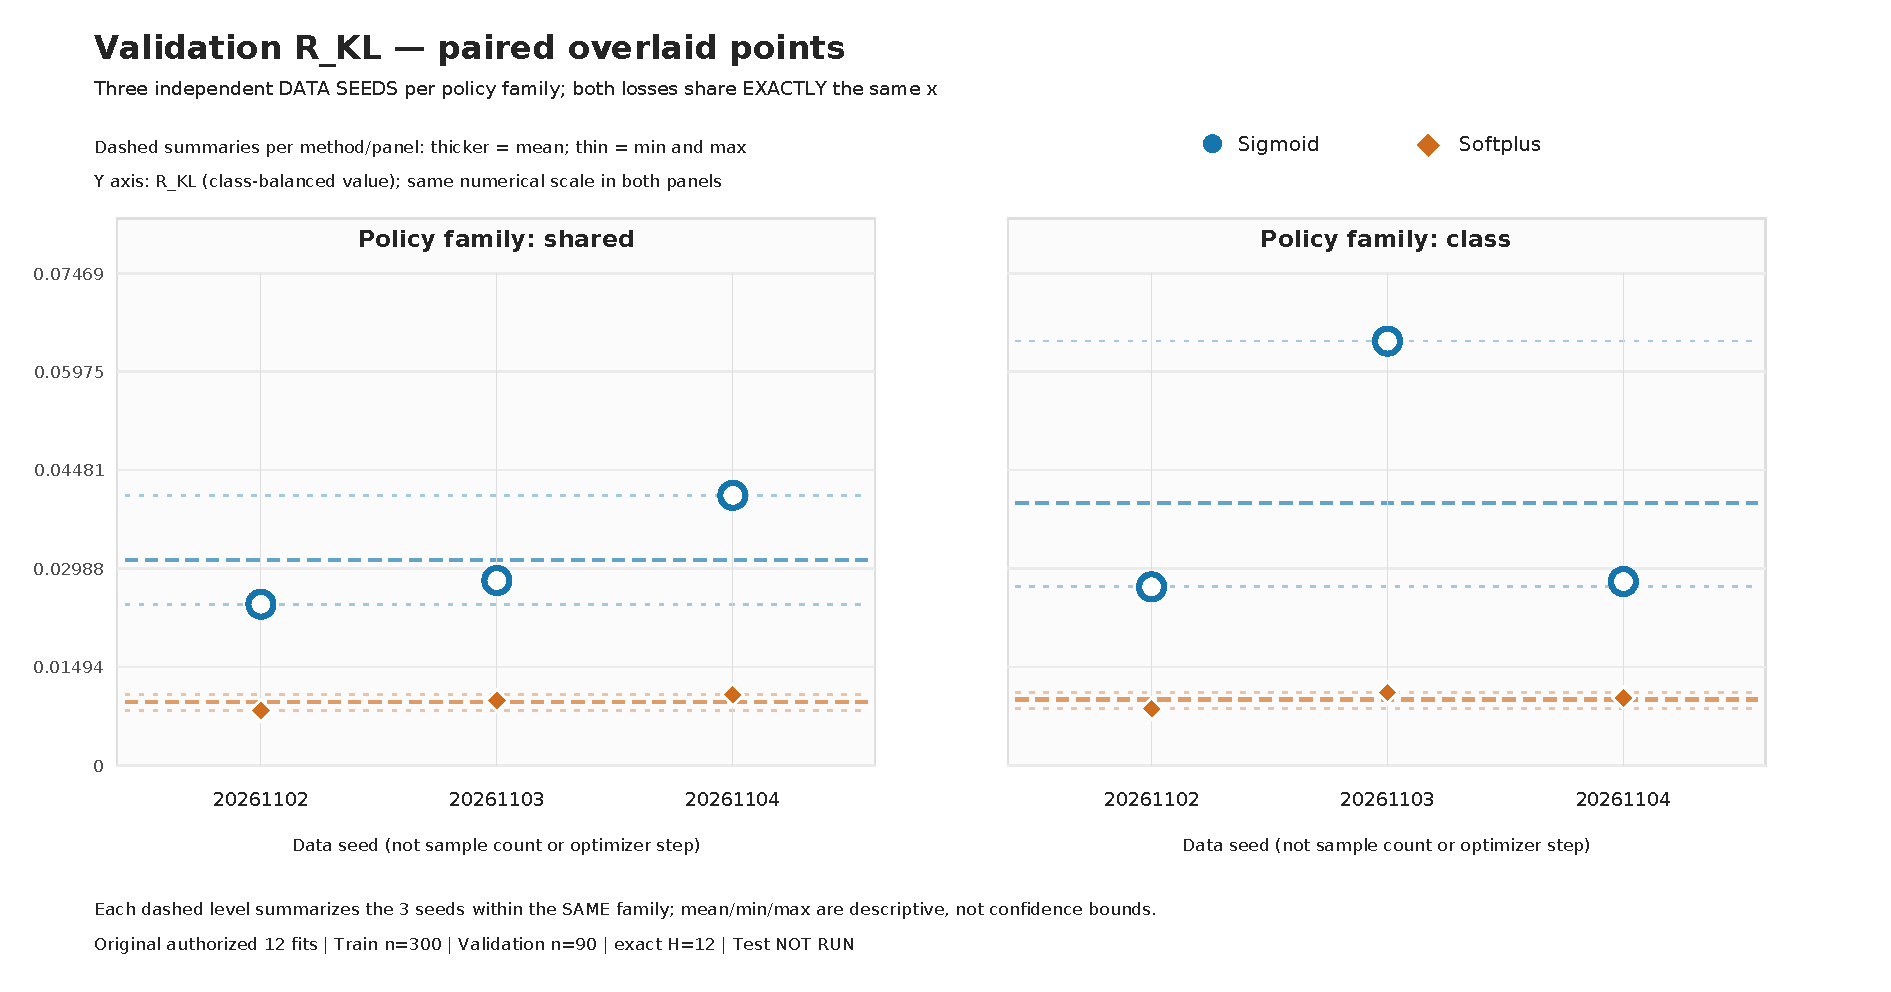
\includegraphics[width=0.98\linewidth]{code/experiments/ch4_loss_controlled_comparison/figures/phase2_tex/phase2_validation_R_KL_six_pairs.pdf}
\caption{تراکم مبتنی بر واگرایی کولبک--لایبلر در مجموعه اعتبارسنجی، با هم‌مکانی افقی دو روش در هر بذر و خطوط چین کمینه، میانگین و بیشینه هر روش و خانواده سیاست. مقادیر کمتر به معنای تراکم بیشتر حول مراکز کلاس است.}
\label{fig:ch4-e13-validation-r_kl}
\end{figure}

\begin{figure}[htbp]
\centering
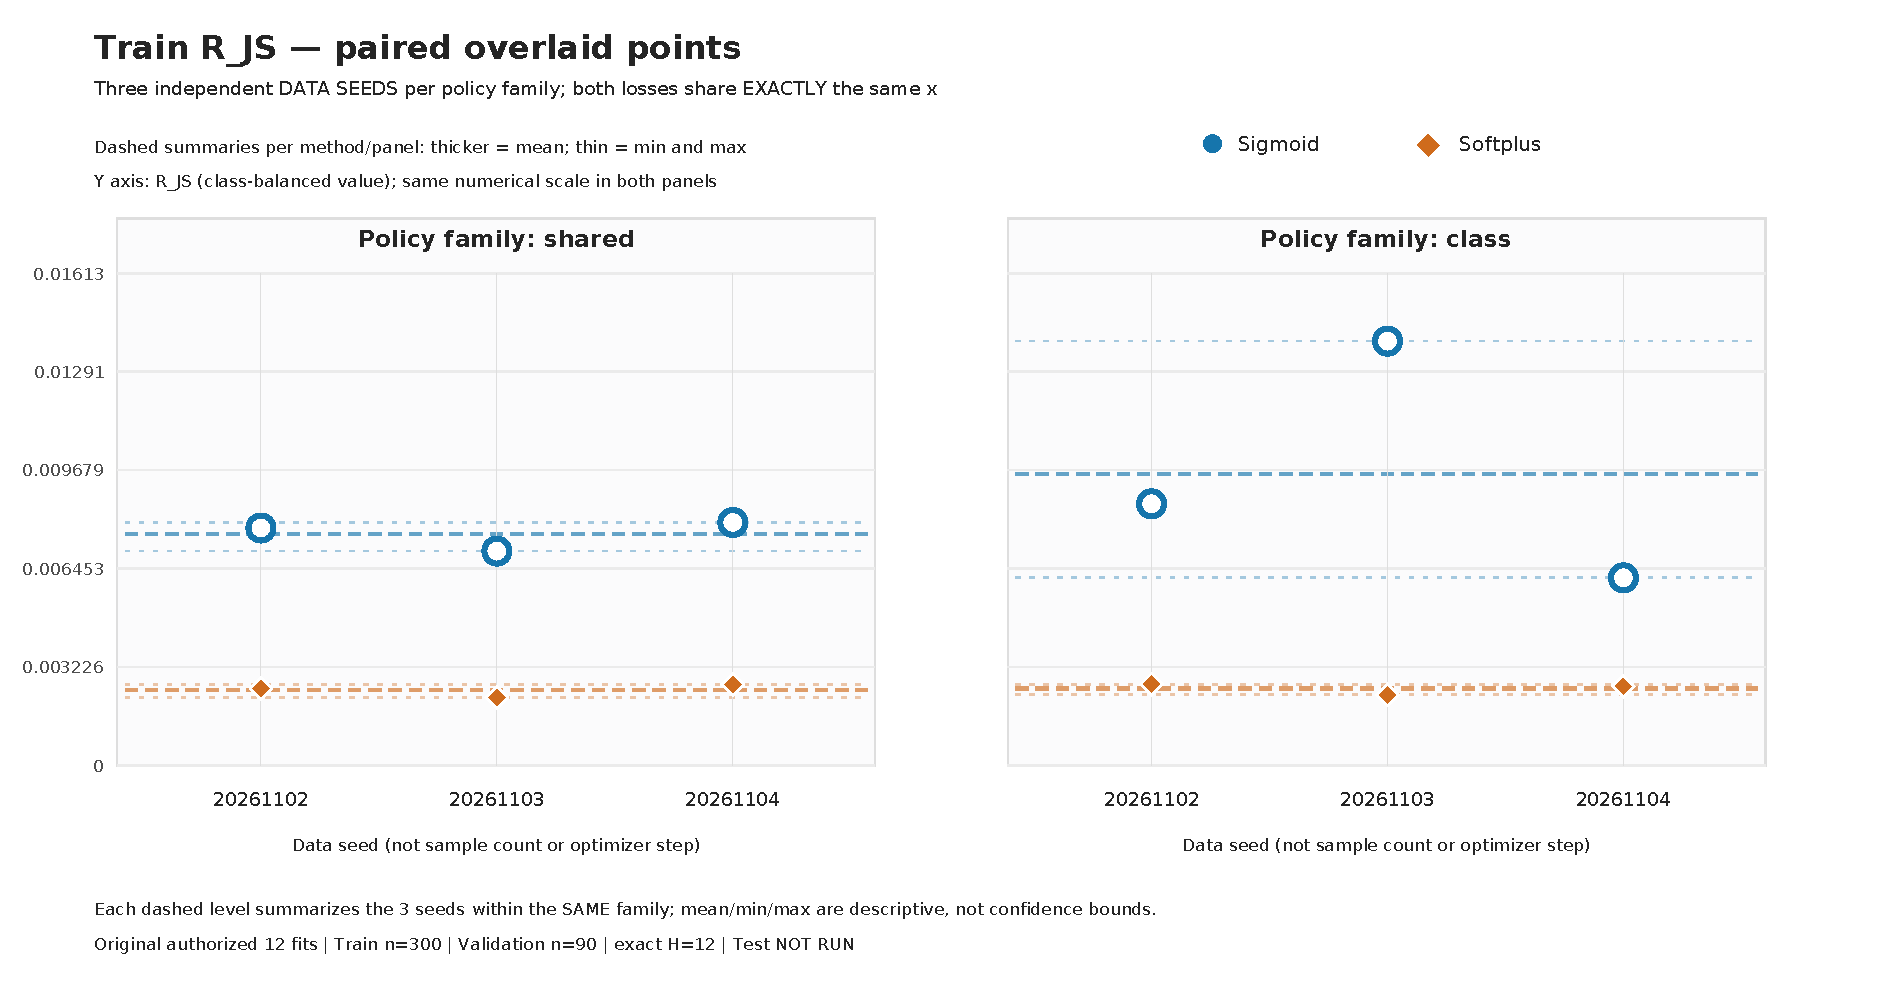
\includegraphics[width=0.98\linewidth]{code/experiments/ch4_loss_controlled_comparison/figures/phase2_tex/phase2_train_R_JS_six_pairs.pdf}
\caption{تراکم مبتنی بر واگرایی جنسن--شنون در مجموعه آموزش، با هم‌مکانی افقی دو روش در هر بذر و خطوط چین کمینه، میانگین و بیشینه هر روش و خانواده سیاست. مقادیر کمتر به معنای تراکم بیشتر حول مراکز کلاس است.}
\label{fig:ch4-e13-train-r_js}
\end{figure}

\begin{figure}[htbp]
\centering
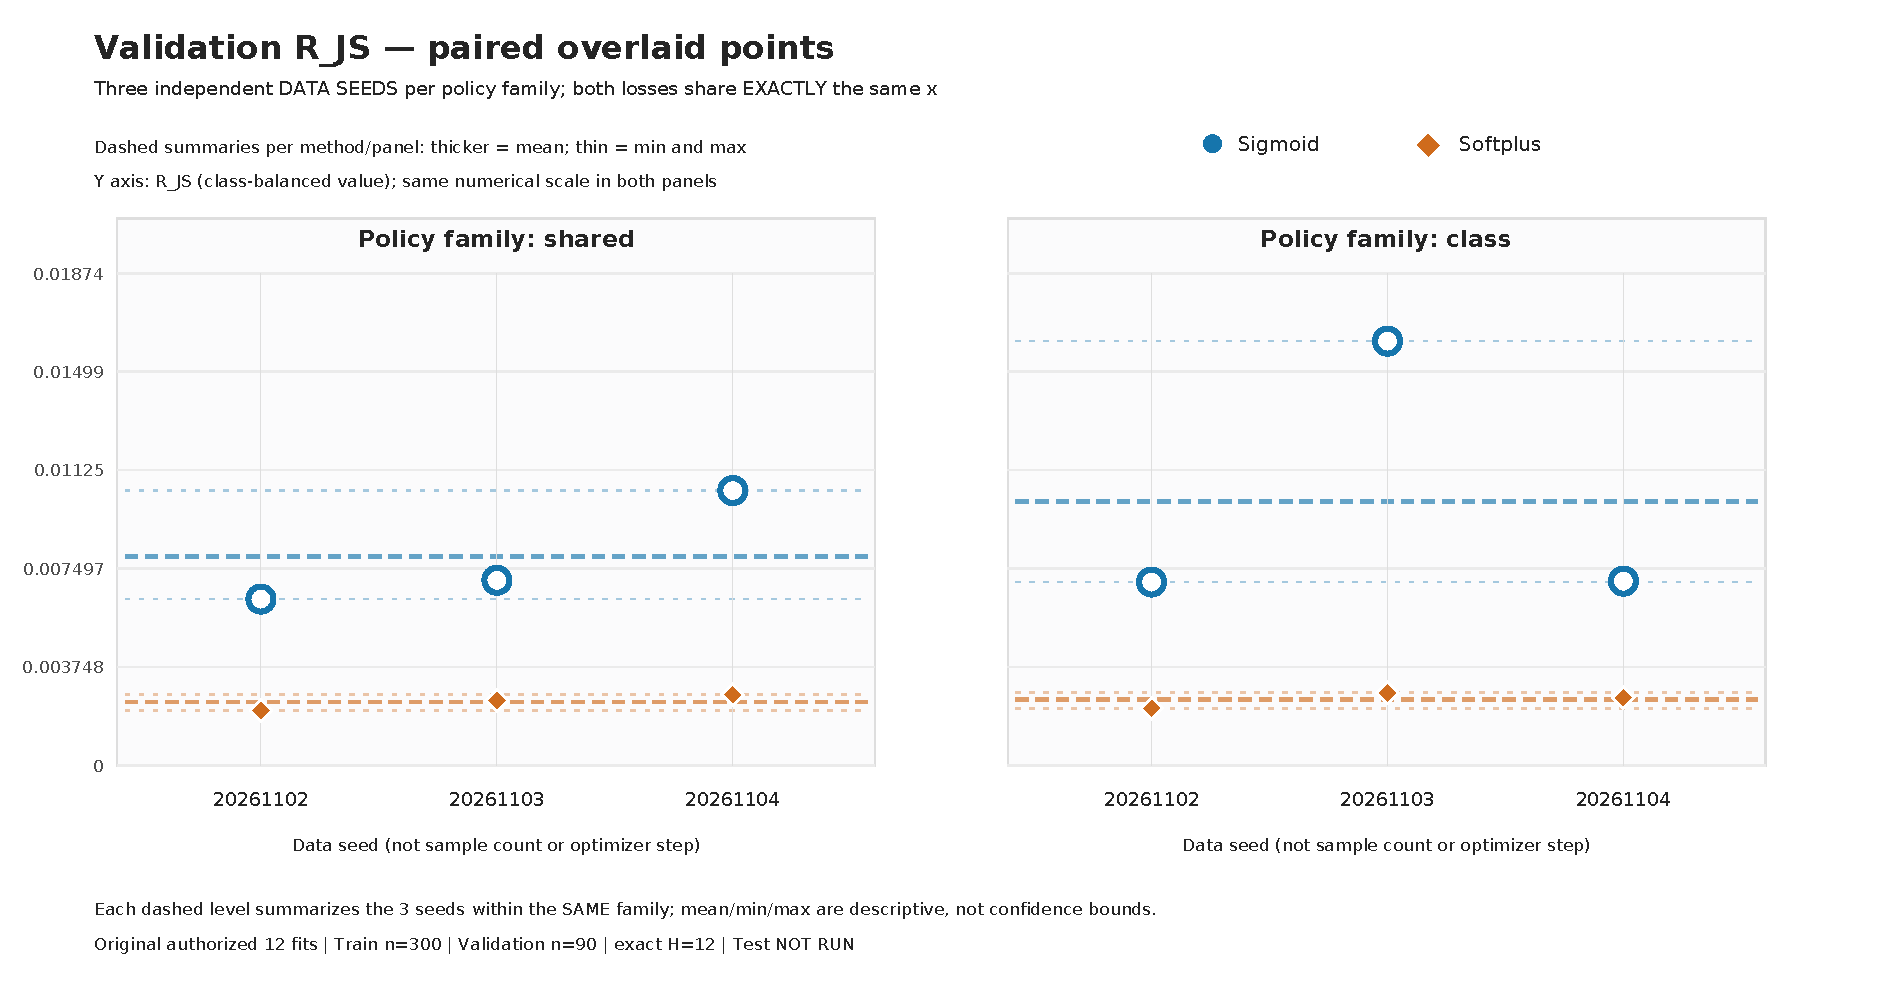
\includegraphics[width=0.98\linewidth]{code/experiments/ch4_loss_controlled_comparison/figures/phase2_tex/phase2_validation_R_JS_six_pairs.pdf}
\caption{تراکم مبتنی بر واگرایی جنسن--شنون در مجموعه اعتبارسنجی، با هم‌مکانی افقی دو روش در هر بذر و خطوط چین کمینه، میانگین و بیشینه هر روش و خانواده سیاست. مقادیر کمتر به معنای تراکم بیشتر حول مراکز کلاس است.}
\label{fig:ch4-e13-validation-r_js}
\end{figure}

\begin{figure}[htbp]
\centering
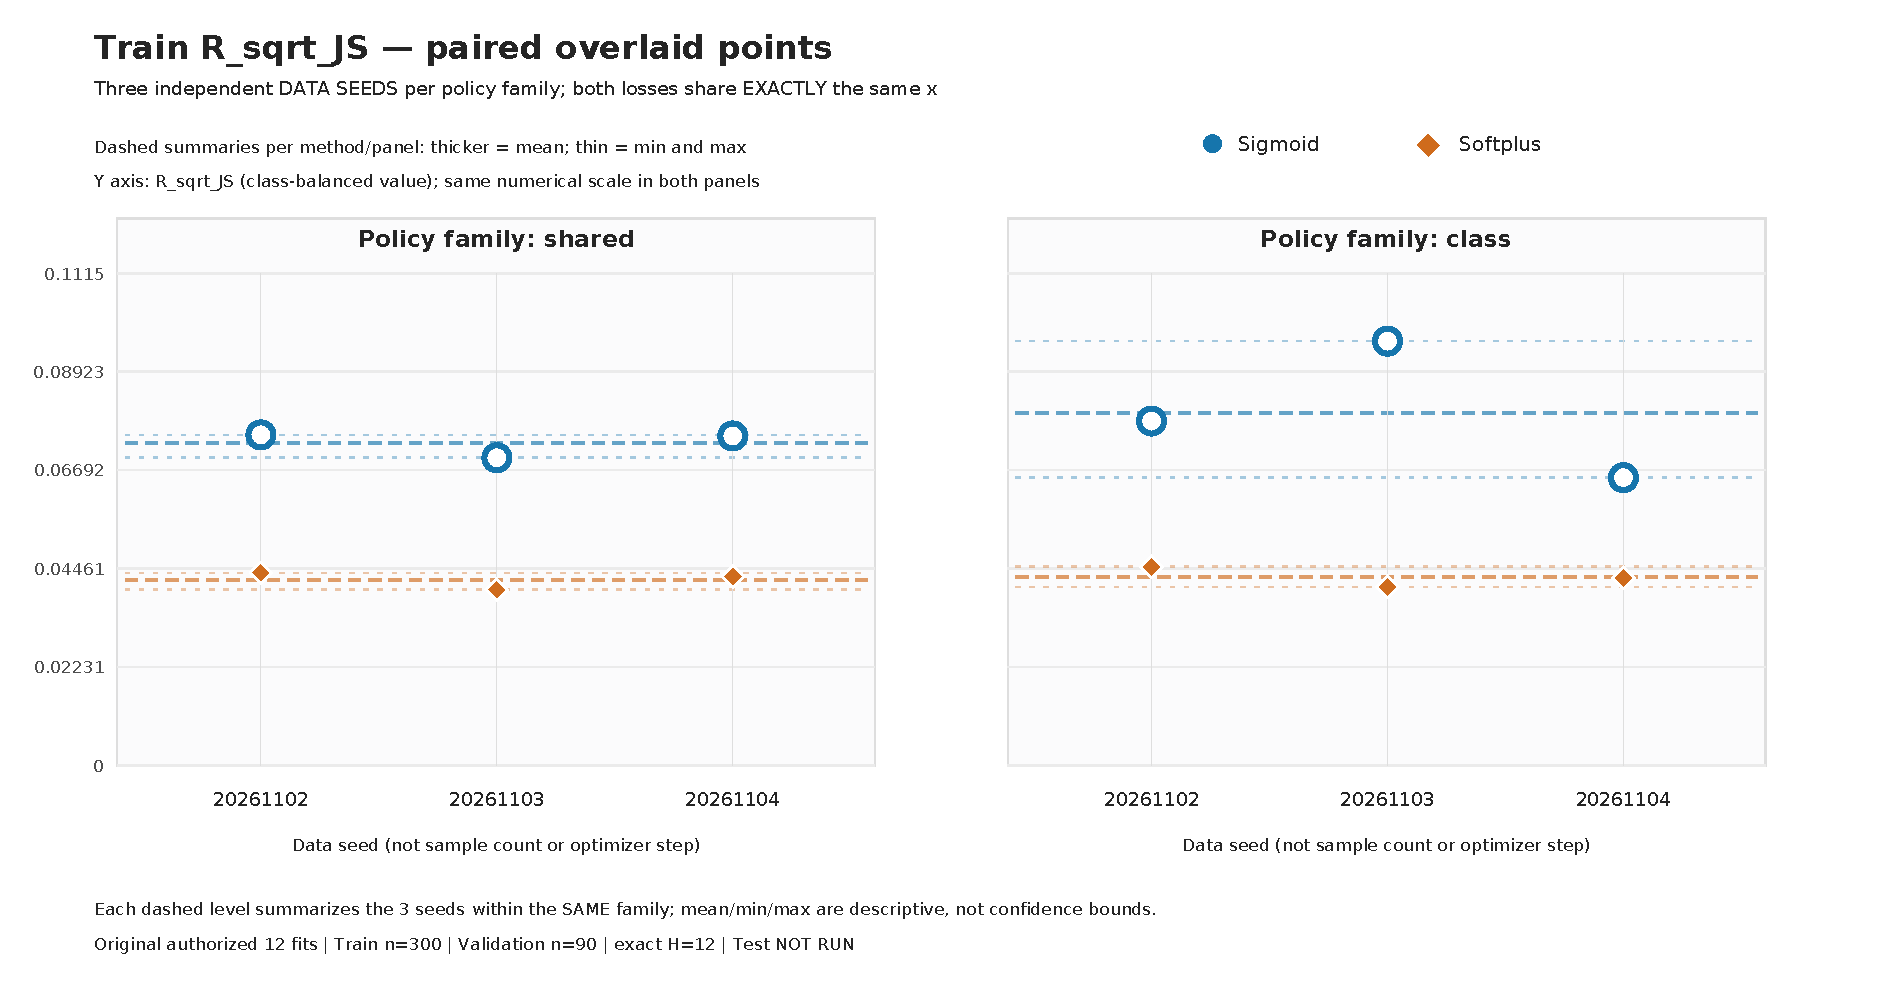
\includegraphics[width=0.98\linewidth]{code/experiments/ch4_loss_controlled_comparison/figures/phase2_tex/phase2_train_R_sqrt_JS_six_pairs.pdf}
\caption{تراکم مبتنی بر ریشه واگرایی جنسن--شنون در مجموعه آموزش، با هم‌مکانی افقی دو روش در هر بذر و خطوط چین کمینه، میانگین و بیشینه هر روش و خانواده سیاست. مقادیر کمتر به معنای تراکم بیشتر حول مراکز کلاس است.}
\label{fig:ch4-e13-train-r_sqrt_js}
\end{figure}

\begin{figure}[htbp]
\centering
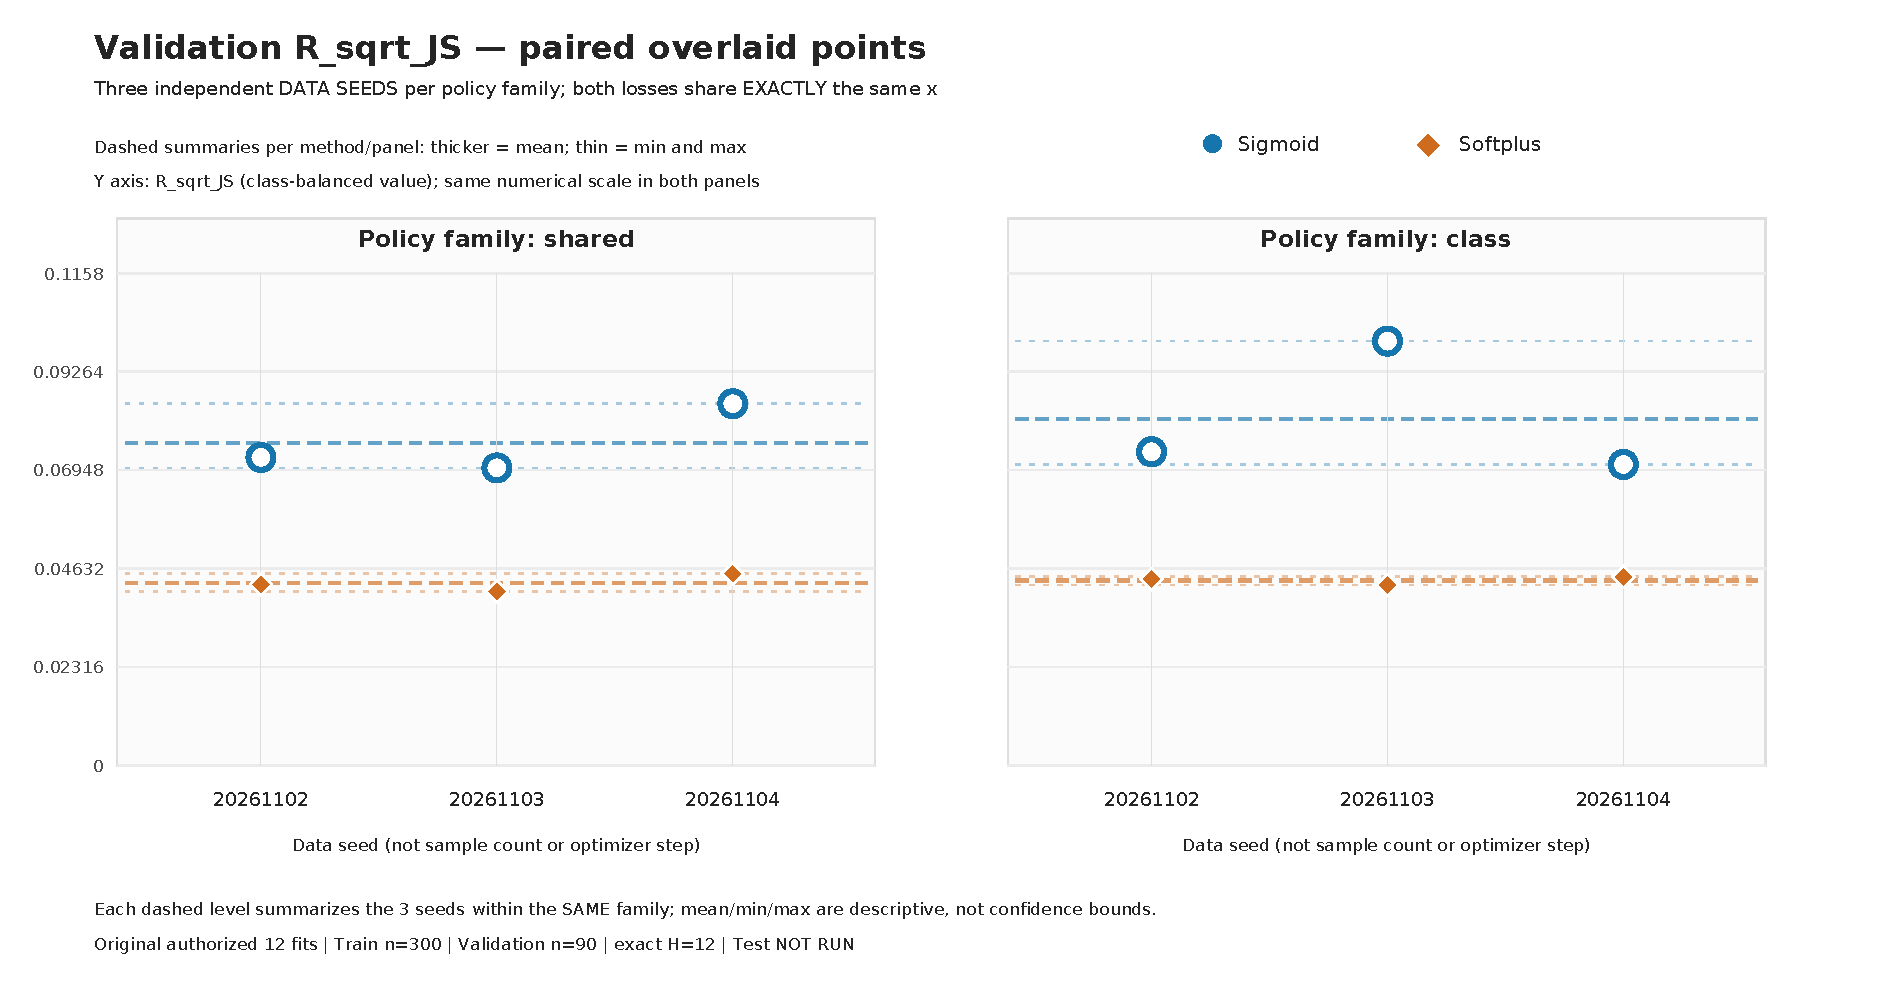
\includegraphics[width=0.98\linewidth]{code/experiments/ch4_loss_controlled_comparison/figures/phase2_tex/phase2_validation_R_sqrt_JS_six_pairs.pdf}
\caption{تراکم مبتنی بر ریشه واگرایی جنسن--شنون در مجموعه اعتبارسنجی، با هم‌مکانی افقی دو روش در هر بذر و خطوط چین کمینه، میانگین و بیشینه هر روش و خانواده سیاست. مقادیر کمتر به معنای تراکم بیشتر حول مراکز کلاس است.}
\label{fig:ch4-e13-validation-r_sqrt_js}
\end{figure}

